% CREATED BY DAVID FRISK, 2016
\chapter{System Development}
\textit{In the following chapter a Top Down approach of the System development is described, with particular emphasis on the hardware development part.}
\section{Overview}
\todo{it should start with a justification and overview of the proposed accelerator}
The entire work is implemented on a PYNQ Z2 board from TUL, based on a Zynq-7000 SoC \cite{paper:31}.

\begin{figure}[!htbp]
\centering
\captionsetup{justification=centering}
\includegraphics[scale=0.35]{./figure/zynq.PNG}
\caption{Zynq 7000 SoC\cite{paper:42}}
\label{fig:zynq}
\end{figure}

The latter is composed of a programmable logic and a processing system, the Programmable logic hosts the accelerator and the relative AXI interconnections while the processing system is in charge of running the software for programming and scheduling correctly the operation on the accelerator.\newline In order to speed-up the development process and use built-in library for the AXI protocol and the DMA transfers, the software is carried out through the PYNQ enviroment of the board \cite{WEBSITE:2} which is based on Python, another reason is that Python has becoma a de facto standard \cite{paper:37}. \\
The usage of Python as basic software allows to easily integrate it with high level Machine Learning API, such as TensorFlow in this case, an end-to-end open source Machine Learning platform \cite{WEBSITE:4}. It has the feature of quantize a post-trained model for different arithmetic precision.\\
Since the aim of the work is focused on the inference process, pre-trained models are needed and TensorFlow Hub \cite{WEBSITE:5} comes in handy for this purpose. It provides already pre-trained Machine Learning models for different domains.

\section{Software}
\todo[inline]{todo -> driver for accelerator and model from tensorflow (also offline quantization) }

\section{System Level}

As it can be seen from \ref{fig:zynq} , it is divided in two big block:
\begin{itemize}
\item Processing System:
The processing system in Figure \ref{fig:sys} referred as \textit{ps7} is in charge of running the OS and the Machine Learning application, as consequence it also runs the necessary software for programming the accelerator registers and the data movement to/from main memory from/to the accelerator.
\item Programmable Logic:
The programmable logic (PL) hosts the entire design, from the accelerator itself to the DMAs and the AXI interconnections.\\ Several single channel DMA have been used instead of using a single DMA with multiple channels, the reason is that the in the PYNQ enviroment only the drivers for the single channel DMA are provided. Furthermore, the Programmable Logic can be divided into:
\begin{itemize}
\item AXI interconnections: IP cores from Xilinx\cite{paper:34}\cite{paper:35} in order to connect and correctly address entities in the Programmable Logic.
\item AXI DMA: IP core from Xilinx \cite{paper:33} which allows data movement between main memory and accelerator memories.
\item DTPU: the actual hardware accelerator.
\item XADC: IP core from Xilinx \cite{paper:32} which allows to measure the temperature of the SoC, the voltages and the currents at runtime.

\end{itemize}

\end{itemize}

\newpage
In the following figure, the schematic of the overall design is presented.
\begin{figure}[!htbp]
\centering
\captionsetup{justification=centering}
\includegraphics[scale=0.97,angle=90]{./figure/system_schematic.pdf}
\caption{System}
\label{fig:sys}
\end{figure}

\section{DTPU, the hardware accelerator}
The hardware accelerator, named \textit{ Dumb Tensor Processing Unit}, is in charge of carring out the computation of the neural network model, exploiting a data-flow architecture on the input data applyng a Fused Multiply Add approach between each unit of the Matrix Multiplication Unit (MXU).

In Figure \ref{fig:logaccel} is presented the Logical block diagram of the accelerator.
\begin{figure}[!htbp]
\centering
\captionsetup{justification=centering}
\includegraphics[scale=0.40]{./figure/logical_view.png}
\caption{Logical view of the accelerator}
\label{fig:logaccel}
\end{figure}

\subsection{Real Implementation}
The work is not focused on developing embedded memories and AXI interfaces, therefore a Xilinx's IP core, which includes all the necessary subcomponents, has been used\cite{paper:43} leading to the actual block diagram which can be observed in the Figure \ref{fig:rtlaccel}.
\begin{figure}[H]
\centering
\captionsetup{justification=centering}
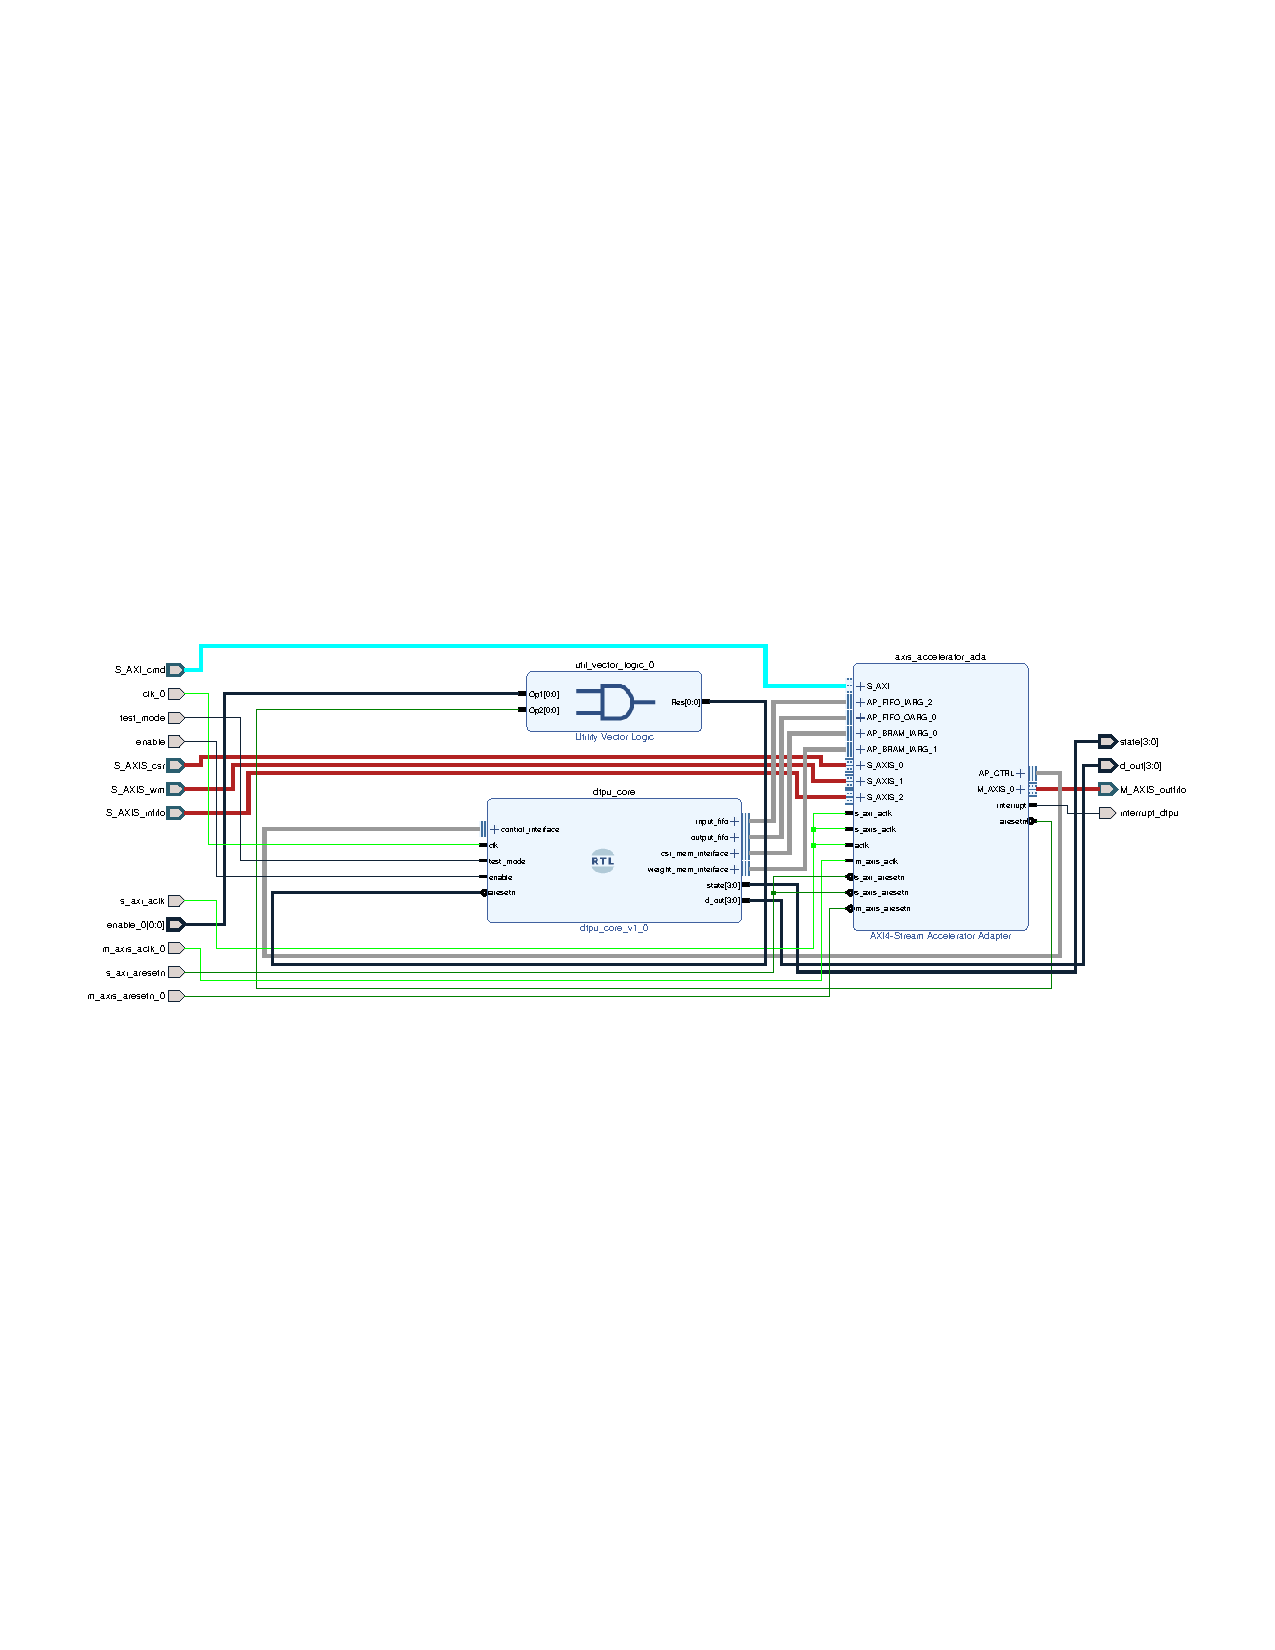
\includegraphics[scale=1,angle=90]{./figure/accelerator_schematic.pdf}
\caption{Real RTL view of the accelerator}
\label{fig:rtlaccel}
\end{figure} 
The latter has allowed to completely focus the work on the DTPU core.
\newpage
\subsection{Axi accelerator adapter}
\subsection{DTPU core}

\subsubsection{Matrix Multiplication Unit}








